\documentclass[12pt,a4paper,english]{article}
\usepackage{times}
\usepackage[utf8]{inputenc}
\usepackage{babel,textcomp}
\usepackage{mathpazo}
\usepackage{mathtools}
\usepackage{amsmath,amssymb}
\usepackage{ dsfont }
\usepackage{listings}
\usepackage{graphicx}
\usepackage{float}
\usepackage{epsfig,floatflt}
\usepackage{subfig} 
\usepackage[colorlinks]{hyperref}
\usepackage[hyphenbreaks]{breakurl}
\usepackage[usenames,dvipsnames,svgnames,table]{xcolor}
\usepackage{textcomp}
\definecolor{listinggray}{gray}{0.9}
\definecolor{lbcolor}{rgb}{0.9,0.9,0.9}
\lstset{backgroundcolor=\color{lbcolor},tabsize=4,rulecolor=,language=python,basicstyle=\scriptsize,upquote=true,aboveskip={1.5\baselineskip},columns=fixed,numbers=none,showstringspaces=false,extendedchars=true,breaklines=true,
prebreak=\raisebox{0ex}[0ex][0ex]{\ensuremath{\hookleftarrow}},frame=single,showtabs=false,showspaces=false,showstringspaces=false,identifierstyle=\ttfamily,keywordstyle=\color[rgb]{0,0,1},commentstyle=\color[rgb]{0.133,0.545,0.133},stringstyle=\color[rgb]{0.627,0.126,0.941},literate={å}{{\r a}}1 {Å}{{\r A}}1 {ø}{{\o}}1}

% Use for references
%\usepackage[sort&compress,square,comma,numbers]{natbib}
%\DeclareRobustCommand{\citeext}[1]{\citeauthor{#1}~\cite{#1}}

% Fix spacing in tables and figures
%\usepackage[belowskip=-8pt,aboveskip=5pt]{caption}
%\setlength{\intextsep}{10pt plus 2pt minus 2pt}

% Change the page layout
%\usepackage[showframe]{geometry}
\usepackage{layout}
\setlength{\hoffset}{-0.5in}  % Length left
%\setlength{\voffset}{-1.1in}  % Length on top
\setlength{\textwidth}{450pt}  % Width /597pt
%\setlength{\textheight}{720pt}  % Height /845pt
%\setlength{\footskip}{25pt}

\newcommand{\VEV}[1]{\langle#1\rangle}
\title{FYS4150 - Project 1}
\date{}
\author{ Kristoffer Langstad\\ \textit{krilangs@uio.no}}

\begin{document}%\layout
\maketitle
\begin{abstract}
In this project we look at different numerical algorithms to solve the one-dimensional Poisson equation with Dirichlet boundary conditions. We solve this equation by approximating through a Taylor expansion to a set of linear equations. This is then solved with two different algorithms; using Gaussian elimination and LU-decomposition on a tridiagonal matrix. We also look at two different cases for the Gaussian elimination method. The end goal is to see how the CPU time and relative error, compared to an analytical solution, changes when using different algorithms and step sizes. Normally we expect that with decreasing step size $h$, the numerical solution would converge closer to the analytical solution. This is not the case here as we get the best results for a step size of $h\approx10^{-6}$ for the Gaussian elimination method. For the LU-decomposition we ran out of memory when computing with a step size larger than $10^{4}$. The Gaussian elimination is also more CPU friendly since the number of floating point operations (FLOPS) for the general algorithm goes as $\mathcal{O}(8n)$, and the special algorithm goes as $\mathcal{O}(4n)$. The LU-decomposition on the other hand goes as $\mathcal{O}(\frac{2}{3}n^3)$ and takes a lot of CPU usage.
\end{abstract}

\section{Introduction}
Differential equations are very powerful tools for explaining and calculating physical problems. Most of these are unfortunately difficult to solve analytically. So we have to use numerics to solve them. Solving them numerically is much easier and much more efficient than trying to solve them analytically. The use of these differential equations in numerics are becoming more and more important today. So to study these are very important to further understand physics.

In this project we are trying to solve the one-dimensional Poisson equation, which is a second order differential equation $-u^{\prime\prime}(x)=f(x)$, numerically. For us to solve this equation we rewrite Poisson's equation as a set of linear equations with Dirichlet boundary conditions. In the program we use memory allocation when we work with matrices with different dimensions to speed up the programing time. To solve the set of linear equations we will use Gaussian elimination and LU-decomposition, and compare the solutions we get from them. Then we compare with a known analytical solution. We also look at the number of floating point operations (FLOPS) for the different algorithms, which have a major effect on the run time of the program. 

First we discretize and derive a finite difference scheme to approximate the second derivative. Then we derive the algorithms to be used and implement them into our program with the necessary boundary and initial conditions. The results we get are then compared to each other for different number of grid points $n$ to see which algorithm has the fastest CPU time and best accuracy in relation to the analytical solution. Then we analyze the results and discuss them. Lastly we come up with a conclusion to the project.


\section{Methods}
\subsection{Poisson equation}
In three dimensions we have Poisson's equation for the electrostatic potential $\Phi$ as 
\begin{equation}
\label{eq:3D_poisson}
\nabla^2\Phi = -4\pi\rho(\textbf{r}),
\end{equation}
where $\rho(\textbf{r})$ is a localized charge distribution. We are looking at a one-dimensional case for a spherically symmetric $\Phi$ and $\rho(\textbf{r})$. Equation \ref{eq:3D_poisson} can then be written as 
\begin{equation}
\label{eq:1D_poisson}
\frac{1}{r^2}\frac{d}{dr}\left(r^2\frac{d\Phi}{dr}\right)=-4\pi\rho(r).
\end{equation}
This can then be rewritten with a substitution $\Phi(r)=\frac{\phi(r)}{r}$ as 
\begin{equation}
\label{eq:rewrite}
\frac{d^2\phi}{dr^2}=-4\pi r\rho(r).
\end{equation}
Then we let $\phi\rightarrow u$ and $r\rightarrow x$ so our one-dimensional Poisson equation can be written as
\begin{equation}
\label{eq:1DPoisson}
-u^{\prime\prime}=f(x),
\end{equation}
where $f(x)=-4\pi x\rho(x)$ is an inhomogeneous source term. The equation we are solving in this project is the one-dimensional Poisson equation (\ref{eq:1DPoisson}) with $x\in(0,1)$ and Dirichlet boundary conditions $u(0)=u(1)=0$.

\subsection{Gaussian elimination}
Poisson's equation (\ref{eq:1DPoisson}) needs to be discretized. We start be approximating the second derivative with a Taylor expansion and discretization of $u \rightarrow v_i$ as
\begin{equation}
\label{eq:approx}
-\frac{v_{i+1}-2v_i+v_{i-1}}{h^2}+\mathcal{O}(h^2)=f(x_i)=f_i,
\end{equation}
where $h=\frac{1}{n+1}$ is the step length and $i=1,...,n$. Define grid points as $x_i=ih$ from $x_0=0$ to $x_{n+1}=1$. We also set boundary conditions $v_0=v_{n+1}=0$. The approximation can further be expressed generally as:
\begin{equation}
\label{eq:approx_gen}
2v_i-v_{i+1}-v_{i-1}=h^2f_i
\end{equation}
From the boundary conditions we get that for $i=0$ and $i=n+1$,which are the end points, we get 0. For the other elements we get:
\begin{align*}
i=1:&\quad 2v_1-v_{2}-v_{0}=h^2f_1\\
i=2:&\quad 2v_2-v_{3}-v_{1}=h^2f_2\\
&\qquad\cdots\\
i=n:&\quad 2v_n-v_{n+1}-v_{n-1}=h^2f_n
\end{align*}
This is a set of linear equations which can be written as
\begin{equation}
\label{eq:lin_eq}
\textbf{A}\textbf{v}=\tilde{\textbf{y}}.
\end{equation}
Here \textbf{A} is a tridiagonal $n\times n$ matrix where $v_i$ are the diagonal elements, and $v_{i+1}$ and $v_{i-1}$ are the elements along the diagonal both above and below. \textbf{v} is a vector of length $n$ and is what we want to find. $\tilde{y}_i=h^2f_i$ is a vector of length $n$ with known elements. The set of linear equations from equation \ref{eq:lin_eq} we have to solve is then written as:
\begin{equation}
\label{eq:matrix_lin_eq}
\begin{bmatrix}
2 & -1 & 0 & \cdots & 0\\
-1 & 2 & -1 &\ddots & \vdots\\
0 & -1 & 2 & \ddots & 0\\
\vdots & \ddots & \ddots & \ddots & -1\\
0 & \cdots & 0 & -1 & 2
\end{bmatrix}
\begin{bmatrix}
v_1\\
v_2\\
\vdots\\
v_n
\end{bmatrix} = 
\begin{bmatrix}
\tilde{\textbf{y}}_1\\
\tilde{\textbf{y}}_2\\
\vdots\\
\tilde{\textbf{y}}_n
\end{bmatrix}
\end{equation}
Then we rewrite the matrix \textbf{A} in terms of one-dimensional vectors \textbf{a}, \textbf{b} and \textbf{c}. The diagonal elements are $b_i$ of length $n$, while $a_i$ and $c_i$ are the below and above elements of lengths $n-1$ respectively.
We solve this new linear equation by doing a Gaussian elimination, which is more thoroughly explained in the class Lecture notes \cite{notes} (sect:6.4.1). What we do are to do a sequence of operations that reduces the matrix \textbf{A} to a upper-triangular matrix. This method is called forward substitution. Then we do what is called a backward substitution to find a solution to the vector \textbf{v}. Mathematically this looks like this:
\begin{equation}
\label{eq:backward}
v_m = \frac{1}{d_{mm}}\left(\tilde{y}_m-\sum^{n}_{k=m+1}d_{mk}v_k\right)\quad m=n-1, n-2, ..., 1
\end{equation}
We will denote $d$ as the changed diagonal elements in the upper-triangular matrix.

We assume a source term as 
\begin{equation}
\label{eq:source}
f(x)=100e^{-10x}
\end{equation} 
in our calculations of the linear equations (\ref{eq:lin_eq}). We also assume different elements of \textbf{a}, \textbf{b} and \textbf{c} in \textbf{A}. Then we use the forward substitution to find equations for the numerical algorithms:
\begin{align}
\label{eq:d_num}
d_i=b_i-\frac{a_{i-1}c_{i-1}}{d_{i-1}}\\
\label{eq:y_tilde}
\tilde{y}_i = y_i-\frac{a_{i-1}\tilde{y}_{i-1}}{d_{i-1}}
\end{align}
Here we see that both equation \ref{eq:d_num} and \ref{eq:y_tilde} have a common factor $a_{i-1}/d_{i-1}$. We pre-calculate this factor to reduce the number of FLOPS in the forward substitution from 6n to 5n, since the common factor is now just calculated once per iteration. Reducing the number of FLOPS reduces the CPU time of the algorithm calculation.

Then we do the backward substitution of \textbf{v}, which in vector notation becomes:
\begin{equation}
\label{eq:v_back}
v_{i-1} = \frac{\tilde{y}_{i-1}-c_{i-1}v_i}{d_{i-1}}
\end{equation}
The endpoint is calculated as
\[v_n=\frac{\tilde{y}_n}{d_n}.\]
The backward substitution calculation requires 3n FLOPS. So in total this general algorithm, also called Thomas algorithm, requires 8n number of FLOPS. In our program, this algorithm is implemented as:
\begin{lstlisting}
# Forward substitution
for i in range(1, n):
	factor = a[i-1]/d[i-1]
	d[i] = b[i] - (c[i-1]*factor)
	y_tilde[i] = f_vec[i] - (y_tilde[i-1]*factor)

# Backward substitution
v[n-1] = y_tilde[n-1]/d[n-1]
for i in range(n-2, 0, -1):
	v[i] = (y_tilde[i-1] - c[i-1]*v[i+1])/d[i-1]
\end{lstlisting}

The program is run for different sizes of matrices of $10\times 10$, $100\times100$ and $1000\times1000$. The results are then plotted and compared to an analytical solution of the differential equation (\ref{eq:1DPoisson}):
\begin{equation}
\label{eq:analytic}
u(x) = 1-(1-e^{-10})x-e^{-10x}
\end{equation}

\subsection{Special case}
Next we assume that the off-diagonal vectors in \textbf{A}, \textbf{a} and \textbf{c}, are identical to each other and different from \textbf{b}, and that all the elements in the vectors are identical. This creates a special case with a tridiagonal Töplitz matrix. This means that we can specialize our previous algorithm to this special case. Now we can reduce the number of FLOPS in the algorithm, since we can pre-calculate more elements.

The diagonal elements $b_i$ are equal to 2, while the off-diagonal elements $a_i$ and $c_i$ are identical and equal to -1. This means that the $d_i$ elements in equation \ref{eq:d_num}, with new boundary conditions and $d_1=b_1=2$, can be pre-calculated as
\begin{equation}
\label{eq:d_special}
d_i = 2-\frac{1}{d_{i-1}}=\frac{i+1}{i}.
\end{equation}
Equation \ref{eq:y_tilde} for the right hand side can also be reduced since we know $d_i$ to
\begin{equation}
\label{eq:y_special}
\tilde{y}_i = y_i+\frac{(i-1)\tilde{y}_{i-1}}{i}.
\end{equation}
This requires only 2n FLOPS for the forward substitution.

The backward substitution in equation \ref{eq:v_back} can be reduced in the same way to 
\begin{equation}
\label{eq:v_special}
v_{i-1} = \frac{i-1}{i}(\tilde{y}_{i-1}+v_i).
\end{equation}
The endpoint is calculated as for the general case. This backward substitution also only requires 2n FLOPS. So in total we now only need 4n FLOPS when calculating the special case algorithm. So in this special case we only need half the number of FLOPS as in the previous general case. The new specialized algorithm with pre-calculated diagonal elements $d_i$ is now implemented as:
\begin{lstlisting}
# Forward substitution
for i in range(2, n):
	y_tilde[i] = y_tilde[i] + y_tilde[i-1]/d[i-1]

# Backward substitution
v[n-1] = y_tilde[n-1]/d[n-1]
for i in range(n-2, 0, -1):
	v[i] = (y_tilde[i] + v[i+1])/d[i]
\end{lstlisting}

We then run the program (both the general and the special case) for matrices up to $n=10^6$ number of grid points, and compare the CPU times for running the algorithms to each other. The CPU times that are compared are averages over a set number of times run. This is because the CPU times may be different for each calculation.

\subsection{Numerical uncertainties}
Numerical calculations will have uncertainties. In this project we look at the relative error we get when the step size $h$ becomes very small. Here we will look closer to where this limit is for our algorithms and compare them.

We will calculate the relative error as
\begin{equation}
\label{eq:rel_error}
\varepsilon_i=\log_{10}\left(\begin{vmatrix}
\frac{v_i-u_i}{u_i}
\end{vmatrix}\right)\quad i=1,...,n.
\end{equation}
This is function of $\log_{10}(h)$ for function values $u_i$ and $v_i$. The $u_i$ values are from the analytical solution (\ref{eq:analytic}) which is compared separately to the numerical solutions $v_i$ from equations \ref{eq:v_back} and \ref{eq:v_special} for grid points up to $n=10^7$.

From the Taylor expansion in equation \ref{eq:approx} we would expect the error to scale as $h^2$. As the step size decrease we would expect to see the affect of the underflow, and be able to see where the step size is too small such that the error would start to increase.

\subsection{LU-decomposition}
Another form of Gaussian elimination is the LU-decomposition. This is a method which splits our matrix \textbf{A} into a product of a lower (L) triangular matrix and a upper (U) triangular matrix on the form as seen for a $4\times4$ matrix in the Lecture notes \cite{notes} (sect: 6.4.2) as:
\begin{equation}
\label{eq:LU}
\textbf{A}=\textbf{LU}=
\begin{bmatrix}
a_{11} & a_{12} & a_{13} & a_{14}\\
a_{21} & a_{22} & a_{23} & a_{24}\\
a_{31} & a_{32} & a_{33} & a_{34}\\
a_{41} & a_{42} & a_{43} & a_{44}
\end{bmatrix}=
\begin{bmatrix}
1 & 0 & 0 & 0\\
l_{21} & 1 & 0 & 0\\
l_{31} & l_{32} & 1 & 0\\
l_{41} & l_{42} & l_{43} & 1
\end{bmatrix}
\begin{bmatrix}
u_{11} & u_{12} & u_{13} & u_{14}\\
0 & u_{22} & u_{23} & u_{24}\\
0 & 0 & u_{33} & u_{34}\\
0 & 0 & 0 & u_{44}
\end{bmatrix}
\end{equation}
A requirement for the LU-decomposition is that the  determinant of our matrix \textbf{A} is non-zero, and \textbf{A} has dimensions $n\times n$.

The LU-decomposition will be solved as 
\begin{equation}
\textbf{Ax}=\textbf{y},
\end{equation}
where \textbf{A} and \textbf{y} are known and \textbf{x} is the solution we want. We then rewrite the equation to
\begin{equation}
\textbf{LUx}= \textbf{y}.
\end{equation}
This equation is further solved in two steps:
\begin{equation}
\label{eq:2_step_LU}
\textbf{Lz}=\textbf{y}\quad \bigwedge\quad \textbf{Ux}=\textbf{z}
\end{equation}
We can easily from equation \ref{eq:LU} see that det(\textbf{L})=1. This further implies that \textbf{L} has an inverse, and we can then solve for \textbf{x} in equation \ref{eq:2_step_LU} as:
\begin{equation}
\label{eq:inv_L}
\textbf{Ux}=\text{L}^{-1}\textbf{z}=\textbf{y}
\end{equation}

To solve the LU-decomposition numerically in Python, we use the library called \textit{scipy.linalg}. The function that solves the LU-decomposition now takes the full matrix \textbf{A} as an argument. This will affect the number of FLOPS. The LU-decomposition of the set of linear equations requires $\frac{2}{3}n^3$ FLOPS. The LU-decomposition is implemented numerically as:
\begin{lstlisting}
import scipy.linalg as scpl
...
LU = scpl.lu_solve(scpl.lu_factor(matrix), func)
\end{lstlisting}
\textit{matrix} is the full matrix \textbf{A} as in equation \ref{eq:matrix_lin_eq}, and \textit{func} is the source function (\ref{eq:source}) multiplied with the step size squared.

Then we compare the mean-time the calculation takes for the LU-decomposition and the relative error, with the mean-times and relative errors for the Thomas and special algorithms for up to $n=10^7$ grid points.

\section{Results}
In Figure \ref{fig:gauss} we see the comparison between the numerical solution with the general Thomas algorithm of the discretized Poisson equation (\ref{eq:approx_gen}) and the analytical solution (\ref{eq:analytic}) for different number of grid points. From that figure we can see by eye that with increasing $n$ (in this case), the numerical solution converges towards the analytical solution. The curves also becomes much smoother with increasing $n$, which means with decreasing step size $h$.

\begin{figure}[htbp]
	\hspace*{-2.5cm}
	\subfloat[Comparison for $n=10$]{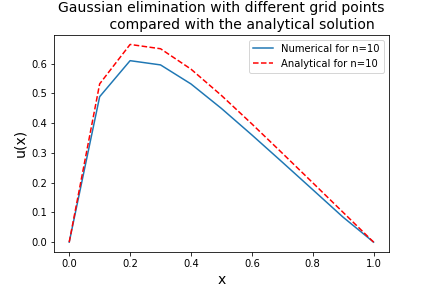
\includegraphics[width=0.45\linewidth]{Gaussian_n=10.png}}
	\subfloat[Comparison for $n=100$]{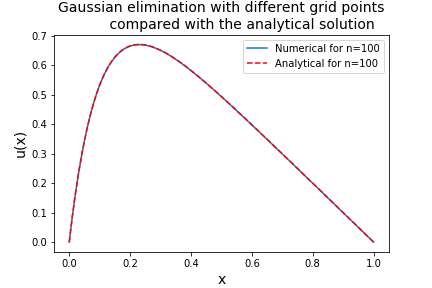
\includegraphics[width=0.45\linewidth]{Gaussian_n=100.png}}
	\subfloat[Comparison for $n=1000$]{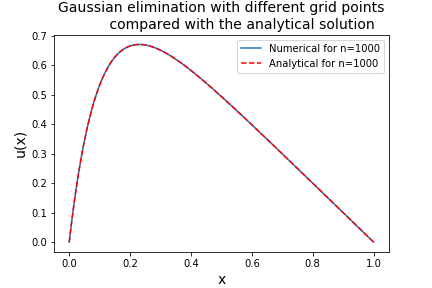
\includegraphics[width=0.45\linewidth]{Gaussian_n=1000.png}}
	\caption{Figures comparing the numerical solution of the Poisson equation (\ref{eq:approx_gen}) to the analytical solution (\ref{eq:analytic}) for different grid points $n=10, 100, 1000$.\label{fig:gauss}}
\end{figure}

In Figure \ref{fig:gauss_LU} we see the comparison between the Gaussian elimination with the Thomas algorithm and the LU-decomposition for different grid points. As for the comparison in Figure \ref{fig:gauss} we see that for increasing $n\in[10,1000]$, the LU-decomposition converges towards the Gaussian solution. The LU-decomposition does not seem to be as good as the Gaussian elimination with the Thomas algorithm, since we see that the Gaussian elimination is much closer to the analytical solution in Figure \ref{fig:gauss}. 

\begin{figure}[htbp]
	\hspace*{-2.5cm}
	\subfloat[Comparison for $n=10$]{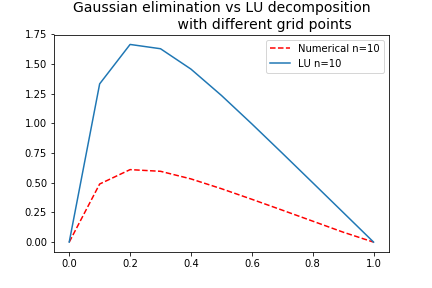
\includegraphics[width=0.45\linewidth]{Gaussian_vs_LU_n=10.png}}
	\subfloat[Comparison for $n=100$]{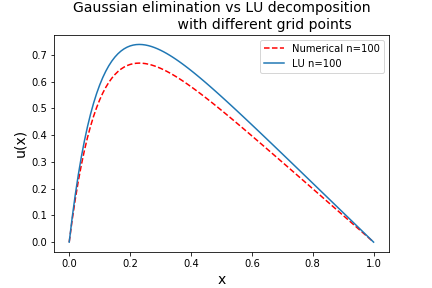
\includegraphics[width=0.45\linewidth]{Gaussian_vs_LU_n=100.png}}
	\subfloat[Comparison for $n=1000$]{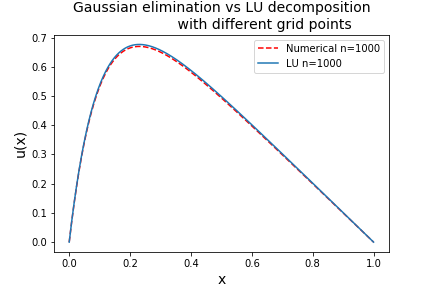
\includegraphics[width=0.45\linewidth]{Gaussian_vs_LU_n=1000.png}}
	\caption{Figures comparing the numerical Thomas algorithm with the LU-decomposition of the Poisson equation for different grid points $n=10, 100, 1000$.\label{fig:gauss_LU}}
\end{figure}

The two figures are only running for $n$ up to 1000. The general and special algorithms of the Gaussian elimination are running for $n$ up to $10^7$, while the LU-decomposition are running for $n$ up to only $10^4$ as we will see when comparing the CPU times and relative errors in Table \ref{tab:times} and \ref{tab:error}. For running the LU-decomposition for $n>10^4$ our computer freezes. This happens since the computer runs out of memory. As we have discussed in the Methods section, we know that the LU-decomposition requires a much higher number of FLOPS than the two other algorithms. This happens since we are using the entire $n\times n$ \textbf{A} matrix and not only some of the elements in \textbf{A}. That means the CPU will use longer to do the decomposition. The FLOPS go as $\frac{2}{3}n^3$ and when we try for $n=5$ we end up with a big matrix. The original computer used have a 8GB memory. So for a matrix of $10^5\times10^5$ matrix we get $10^{10}\times 8$ bytes which is approximately 100GB. This is much much bigger than the computer memory, which causes memory error.

\begin{table}[h!]
%\centering
%\hspace{-1cm}
\begin{tabular}{ |c|c|c|c| }
	\hline \rule{0pt}{13pt}
	Value of n&General [s]&Special [s]&LU-decomposition [s]\\
	\hline \rule{0pt}{13pt}
	$10$&$2.152\cdot10^{-5}$& $9.846\cdot10^{-6}$ & $1.216\cdot10^{-2}$\\
	\hline \rule{0pt}{13pt}
	$10^2$ & $1.904\cdot10^{-4}$ & $9.153\cdot10^{-5}$ & $1.391\cdot10^{-2}$ \\
	\hline \rule{0pt}{13pt}
	$10^3$ & $2.235\cdot10^{-3}$ & $1.156\cdot10^{-3}$ & $2.807\cdot10^{-2}$\\
	\hline \rule{0pt}{13pt}
	$10^4$ & $2.286\cdot10^{-2}$ & $1.056\cdot10^{-2}$ & 7.783\\
	\hline \rule{0pt}{13pt}
	$10^5$ & $2.256\cdot10^{-1}$ & $1.109\cdot10^{-1}$ & $\cdots$\\
	\hline \rule{0pt}{13pt}
	$10^6$ & $2.266$ & $1.054$ & $\cdots$\\
	\hline
\end{tabular}	
\caption{Table with the mean measured times of the different algorithms in seconds for the different grid points.}
\label{tab:times}
\end{table}

In Table \ref{tab:times} we see the measured mean times of running the three mentioned algorithms. We have measured the mean of the times since each time we run the algorithms the single times will be different each time. This is because the CPU usage will change each time a algorithm is ran. This comes from that the CPU may be doing other things in the background that will affect the run times. From the time-table we see that the specialized algorithm of the Töplitz matrix is the fastest as expected, while the LU-decomposition is the slowest. This corresponds well with the number of FLOPS required for each algorithm. The specialized have the least amount of required FLOPS (4n), while the LU-decomposition requires the most FLOPS ($\frac{2}{3}n^3$). So we clearly see that the number of FLOPS in an algorithm will affect the CPU run time. For the LU-decomposition we got memory error with $n=5$ and bigger. Already at $n=4$ we see in Table \ref{tab:times} that the time have increased a lot compared to the two other algorithms at this stage.

\begin{table}[h!]
	%\centering
	%\hspace{-1cm}
	\begin{tabular}{ |c|c|c|c| }
		\hline \rule{0pt}{13pt}
		Value of n&General &Special &LU-decomposition \\
		\hline \rule{0pt}{13pt}
		$10$&$1.62611\cdot10^{-1}$& $7.93264\cdot10^{-2}$ & $1.50265$\\
		\hline \rule{0pt}{13pt}
		$10^2$ & $1.06807\cdot10^{-2}$ & $8.32917\cdot10^{-4}$ & $1.04250\cdot10^{-1}$ \\
		\hline \rule{0pt}{13pt}
		$10^3$ & $1.00279\cdot10^{-3}$ & $8.33329\cdot10^{-6}$ & $1.00418\cdot10^{-2}$\\
		\hline \rule{0pt}{13pt}
		$10^4$ & $9.96191\cdot10^{-5}$ & $8.33337\cdot10^{-8}$ & $1.00042\cdot10^{-3}$\\
		\hline \rule{0pt}{13pt}
		$10^5$ & $9.95577\cdot10^{-6}$ & $8.33680\cdot10^{-10}$ & $\cdots$\\
		\hline \rule{0pt}{13pt}
		$10^6$ & $8.40358\cdot10^{-7}$ & $6.67281\cdot10^{-11}$ & $\cdots$\\
		\hline \rule{0pt}{13pt}
		$10^7$ & $2.98380\cdot10^{-6}$ & $2.22126\cdot10^{-10}$ & $\cdots$\\
		\hline
	\end{tabular}	
	\caption{Table with the maximum relative errors for the three algorithms calculated from equation \ref{eq:rel_error}.}
	\label{tab:error}
\end{table}
In Table \ref{tab:error} we see the maximum relative errors for the three algorithms used compared to the analytical solution. For all three algorithms we see that for increasing $n$, which means decreasing step size $h$, we see that the relative error decreases. This is as expected. When we go higher than $n=10^6$ we see that the relative error starts to increase. This means that there is a limit for how small step size we can use. The reason for this is that on computers there are limitations for how high and low numbers can be represented. So when we approach to this limit, we get round off errors that affect our results. In Figure \ref{fig:rel_error} we have plotted the relative error as a function of $\log_{10}(h)$ for the general and special algorithms. There we see that for decreasing step size up until $n=10^6$ the relative error decreases. After that the relative error increases.

From Table \ref{tab:error} for the LU-decomposition we see that the relative error is much bigger than for the others, especially for $n=10$. We can also see this from Figure \ref{fig:gauss_LU} where the curve for the LU-decomposition is much further apart from the analytical than in Figure \ref{fig:gauss}. We would expect that the LU-decomposition would be more or less as good the other algorithms. So there might be something wrong with the code for the LU-decomposition.
\begin{figure}[htbp]
	%\hspace*{-2.5cm}
	\subfloat[]{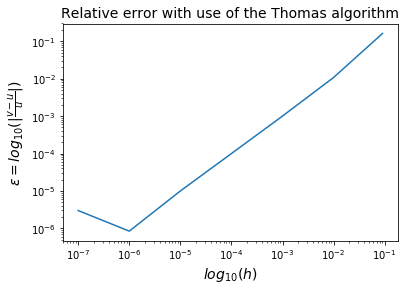
\includegraphics[width=0.5\linewidth]{Error_general.png}}
	\subfloat[]{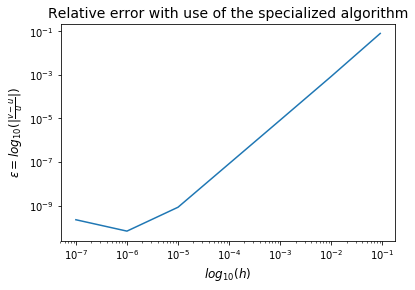
\includegraphics[width=0.5\linewidth]{Error_special.png}}
	\caption{Relative error as functions of $\log_{10}(h)$ .\label{fig:rel_error}}
\end{figure}

\section{Conclusion}
The reason for this project was to solve the Poisson equation by first discretization and then to solve it with different Gaussian elimination methods, and compare the results from these algorithms. We have studied the effect different step sizes have on our numerical results by looking at the CPU time of the calculations, and the relative error between the algorithms and the analytical solution. 

We have come to the conclusion that for numerical calculations on the computer there exists a limit for how small step sizes we can use until the results are negatively affected. For each algorithm we have seen that the CPU time is dependent on the required number of FLOPS. With $n$ bigger than $10^4$ we saw that LU-decomposition is no longer useful, since all we got was memory error. So arithmetic underflow may cause loss of precision and may have influence on our results.

For the comparison with the analytical solution we see that for even smaller $n$ we get good precision with short CPU time. Specially in Figure \ref{fig:gauss} we see that for not so big $n$ the curves stay more or less on top of each other, at least be eye.

An improvement for later use could be to do the main code in C++, which will most likely have a greater affect on the calculations we are going to do later in the course.

\section{Appendix}
Link to GitHub repository:
\url{https://github.com/krilangs/FYS4150/tree/master/Project1}

\begin{thebibliography}{}
\bibitem[1]{notes} 
Hjorth-Jensen, M. (2015). \textit{Computational Physics - Lecture notes Fall 2015}

\end{thebibliography}

\end{document}
